\documentclass[12pt]{article}

\usepackage{fullpage}
\usepackage{graphicx}
\usepackage{hyperref}
\usepackage{listings}
\usepackage{multirow}
\usepackage{pdflscape}

\begin{document}

\title{
\includegraphics[height=0.3\textheight]{logo}}
\date{}
\maketitle

\vfill

\begin{center}
    \begin{tabular}{lr}
        Yun Chan Han & \url{ychani@umich.edu}\\
        Jiqing Jiang & \url{jqjiang@umich.edu}\\
        Alex LaBerge & \url{alaberge@umich.edu}\\
        Jacob Perrin & \url{tcperrin@umich.edu}\\
        Alec Ten Harmsel & \url{talec@umich.edu}\\
    \end{tabular}
\end{center}

\newpage

\tableofcontents

\newpage

\section{Summary}
Every year around 500 people are killed by law enforcement personnel. In 2015,
especially, people are wondering how many of these deaths were preventable. One
classic way to ensure that all protocols were being followed has been a police
body camera. However, these are often expensive (\$800 - \$1200 each
\cite{cam}) and have serious privacy concerns for the police officers. If the
body cameras are always on, you might record private moments that an officer
does not want his superiors seeing. However, if we give the officer a way to
turn it on and off and police abuse may start occurring. The proposed device
would be an upgrade to the current system: a way to measure and record police
weapon usage as well as a way to keep track of the officers and their behavior
when weapons are pulled without violating their privacy.

Compared to the competition, our product will be cheaper and contain better
features to ensure civilian and officer safety while maintaining privacy. This
product, as shown in Figure \ref{fig:installation},  will see use because it hits a middle ground that city officials and
law enforcement officials can agree upon. It will be cost-effective, while also
being robust and hopefully life-saving.

\begin{figure}[h!]
    \centering
    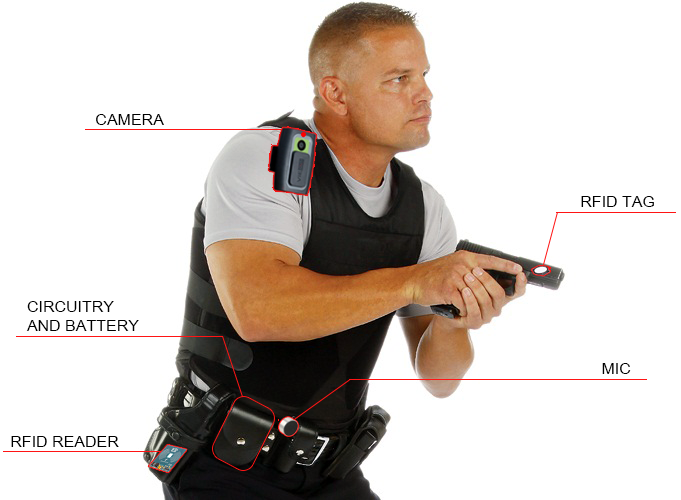
\includegraphics[width=0.9\textwidth]{installation}
    \caption{Overview of Installation}
    \label{fig:installation}
\end{figure}

\section{Description}

This design needs to be cheaper to produce than current body-cam systems as
well as being accurate in how and why it records data (in a manner which keeps
officers' private information private). We do not want to capture the call they
have in the squad car with their wives, but we do want to capture the stop
where a suspect gets out of their car and attempts to attack the officer.
Officers will be more likely to use it for these features. In addition, storing
the amount of footage from body cameras that are always on represents a significant
challenge for police departments\cite{store1,store2}.

Some of the solutions that are already on the market include many more features
than are feasible for the scope of this project. Wolfcom has a product called
the 3rd Eye\cite{third_eye} which has a snapshot button, a screen for seeing
what the camera sees, and HDMI support. However, it comes at a steep price
point of \$475.  However, it does not include streaming and many of the
features seem to be those of a swiss-army-knife of cameras rather than for
stopping police brutality. Also, officers have complete control over the camera
and therefore could abuse the technology. Our solution would have the same
resolution of 1080p at 30fps, while leaving the control up to the environment
and would provide instant feedback to the police station about the officer's
behaviour and safety.

Both of our proposed solutions require a body-mounted camera and a pack located
on the user's hip that interfaces with both the camera and a possible custom
holster. These two designs differ on how they process and store the
incoming data.

In one of the proposed designs, the camera will take a picture once the gun has
been brought up to be fired, as well as taking pictures on each trigger pull.
These pictures will be sent back to the pack on the user's hip and then
wirelessly streamed over to the computer within the squad car. 

In the other proposed design, the camera will start recording video once the
gun has been removed from the holster and will send video to be stored locally
on the officer's hip pack that will be streamed over when a reliable connection
can be established.

In both designs, we will use a GPS device for tracking the officer as well as
synchronizing the video or images with the current time, which is included in
the GPS protocol.

One way we could tell if the gun is being brought up to be fired will be with a
gyroscope attached to the weapon. An alternative to this option would be a
holster mechanism which will tell if a gun has been pulled by checking if an
RFID tag can be read. This RFID tag will have a range such that it only reads
the tag if the gun when it is in the holster. If it cannot be read, the gun is
not holstered. The video feed would then begin to record.

The tradeoffs of each design are fairly simple. For the design that takes
pictures, storage would be much easier as would wireless transmission of the
pictures. This design would probably not be as power hungry either, as
streaming data will be a huge consumer of battery. However, if the picture is
blurry or we got a picture at a point where the police officer is not facing
the suspect, we are out of luck. We also would not likely have synchronized
sound. The video design, on the other hand, will be much harder to implement
due to the streaming of video. We would probably need a Linux-based (or other
higher-level ``RTOS'') processor to interface with Wi-Fi as well as to make
streaming easier.  This would be a pain to wake up every time we needed to
start recording on the camera. Due to the fact that we would probably always
need to keep the camera on but not recording, power consumption becomes one of
the bigger problems.  Between constantly keeping the camera on and the amount
of power required to run an RFID reader and microphone algorithm, we could run
into many issues trying to power our device. An alternative would be to
dedicate a processor to this and write an interface which can be on, but not as
power-intensive.  Some of the difficulties of implementing both designs will be
discussed next.

\subsection{Snapshot Solution}

The chief implementation difficulty raised in this solution is mechanically
determining a trigger pull. Gathering, saving, and streaming a small set of
pictures requires much less processing power than video, but may not be as useful
as evidence in the courtroom. Adding streaming capabilities in addition to a
camera on the gun would most likely add enough bulk to the gun that it would
interfere with the ability to handle it.

\subsection{Video Feed Solution}

Any device that streams video consumes a large portion of processing and power.
This would be a challenge for a device that needs to be smaller than 120 x 70 x
20 mm to sit on someone's belt. Also, we would have to interface with a video
encoder/decoder in order to stream efficiently, and increasing the number of
devices can always lead to problems. This would likely require a separate
processor dedicated solely for this processing, as it would have to be on only
when the video is being recorded and sent in order to conserve power. This
means we would have to interface between processors in addition to the other
issues.

\subsection{Camera Mount Solution}

Most of mounting in the industry use clips to attach a camera on a body. Among
different clipping mounts, positions where they are clipped to vary. We have
found three common positions where a camera can be clipped to: glasses, chest,
and shoulder. After comparing pros and cons of each, we have decided to use the
clip mounted to shoulder as our mount type as it has moderate accuracy and
stability without much obstruction. The comparisons of these options are
summarized in the table below.

\begin{table}[h!]
    \centering
    \caption{Comparison of different types of camera mounts}
    \begin{tabular}{|l|l|c|}
        \hline
        \textbf{Mount Type} & \textbf{Pros and Cons} & \textbf{Mounted Image}\\
        \hline
        & & \\
        Sunglasses Clip & Pros: & \multirow{8}{*}{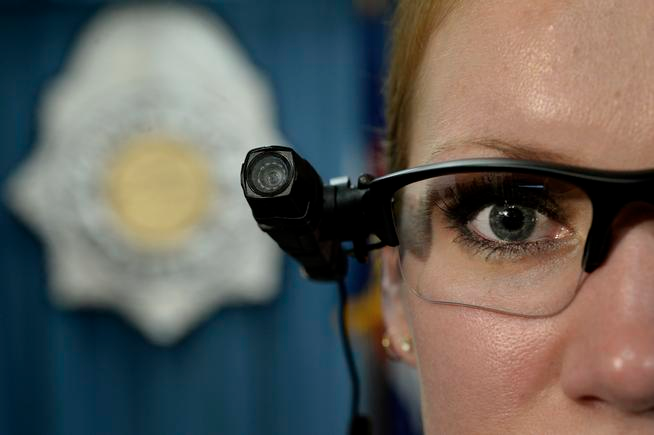
\includegraphics[width=0.3\textwidth]{glasses_mount}}\\
                        & - Camera direction corresponds to LOS & \\
                        & - Most accurate in camera's view & \\
                        & - Stable & \\
                        & & \\
                        & Cons: & \\
                        & - Has to wear glasses & \\
                        & - Can be disturbing & \\
        & & \\
        \hline
        & & \\
        Chest Clip & Pros: & \multirow{8}{*}{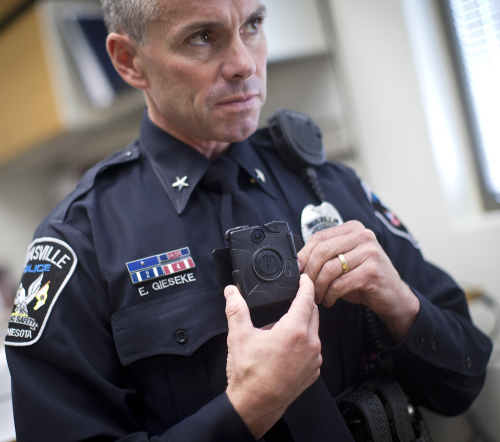
\includegraphics[width=0.3\textwidth]{chest_mount}}\\
                   & - Not disturbing & \\
                   & & \\
                   & Cons:  & \\
                   & - View can be blocked by officer' arms & \\
                   & - Can be unstable upon active movement  & \\
                   & & \\
                   & & \\
                   & & \\
        \hline
        & & \\
        Shoulder Clip & Pros: & \multirow{7}{*}{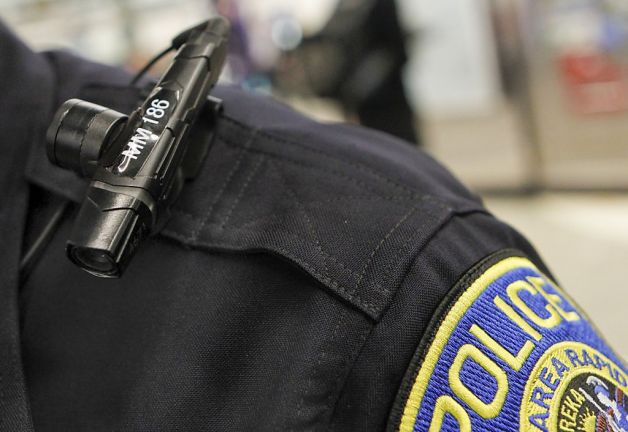
\includegraphics[width=0.3\textwidth]{shoulder_mount}}\\
        (selected) & - Moderately accurate in camera's view & \\
                   & - View is unlikely to be blocked & \\
                   & & \\
                   & Con: & \\
                   & - Can be unstable upon active movement  & \\
                   & & \\
        \hline
    \end{tabular}
    \label{tab:cam_mount}
\end{table}

\subsection{Comparison with Other Products}
Table \ref{tab:fin_comp} contains a feature comparison between our finished
product with other body cameras that are currently available.

\begin{table}[h!]
    \centering
    \caption{Comparison of finished products}
    \begin{tabular}{llll}
        \textbf{Name} & Team Edgy & PatrolEyes SC-DVAI & Wolfcom Vision\\
        \textbf{Price} & \textasciitilde \$300 & \$449 & \$249\\
        \textbf{Video Capacity} & 32 GB & 32 GB & 32 GB\\
        \textbf{Video Resolution} & 1080p & 1080p & 1080p\\
        \textbf{Video Format} & MOV, MPEG-4 & AVI & MOV, MPEG-4\\
        \textbf{Photo Resolution} & 12M & 16M, 12M, 5M, 3M & 16M, 12M, 8M, 5M, 3M\\
        \textbf{Standby Time} & 10 hours & 35 hours & $>$ 5 days\\
        \textbf{Remote Control} & No & Yes & No\\
        \textbf{Field of View} & $120^o$ & $120^o$ & $120^o$\\
        \textbf{Mass} & 100g & 151g & 63g\\
        \textbf{Infrared Camera} & No & Yes & No\\
        \textbf{Dimensions} & 120 x 70 x 20 mm & DVR: 79 x 51 x 22 mm & 74 x 38 x 15 mm\\
                            & & Camera: 55 x 48 x 38 mm & \\
    \end{tabular}
    \label{tab:fin_comp}
\end{table}

\section{Implementation Issues}

The device revolves around two main parts, the belt enclosure and the camera.
The holster sensor will be an RFID reader which, when it cannot read the RFID
tag on the weapon, will send a signal to the main processor. This processor
will be located on the belt in an enclosure along with any other processors we
have. The main processor will then send a signal to begin gathering data
through a video camera that we have attached to the officer. 

The video will be recorded onto an SD card and streamed back when a wireless
signal is available. We are planning on setting up a Raspberry Pi or similar
processor as a wireless access point for Wi-Fi, so we could attach a Wi-Fi
module onto the wearable and stream the video data back over that connection.
This Pi will serve its purpose for our prototype, but the officer's laptop or
in-car wireless module will serve as the server in a final product. We are
choosing Wifi over cell in order to decrease the operating cost of the final
product. Wifi radios are less expensive and often squad cars already contain
internet connections. For officers without a squad car, cellular options can be
provided. However, this will not be included in the scope of this project. This
streaming would likely require a dedicated processor, which would also go in
the hip enclosure. One processor that might be able to work is the TIVA, made
by TI. MAAV, the Michigan Autonomous Aerial Vehicle team, uses TIVAs and USB
webcams to stream HD video, so we figured it is definitely doable on this
platform. The video would be encoded by this chip and then sent over a Wifi
radio with a UART interface.

We will also have a microphone interfaced to the main processor, which will
also cause a record signal to be sent if it detects loud noises. This is to
potentially capture any violent scenarios that do not include a weapon being
drawn. This microphone will probably not save any data, but will instead be
used solely for the purpose of detecting a decibel amplitude above a certain
threshold as a trigger to begin capturing video.

We will also have a Real Time Clock (RTC) on the device, which will be used to
timestamp the videos. To sync the RTC, we will be using a GPS device to get the
time from that protocol. This has an added bonus of also giving us the GPS
coordinates of the police officer. The reason we cannot use solely GPS is that
signal may not be available indoors. This timestamp data will be added as
metadata to the video before it is sent off to be streamed. 

For the camera, we have a few potential devices. We could use a premade camera
that saves data onto an SD card and interface with that, or we could use
something like an IP camera that already has network-level streaming available.
Both of these options are possibilities, but having an IP camera would limit
how low-level we can stay with the camera processing and will probably force us
into using something like embedded Linux (or worse). The foreseen issue with
embedded Linux is the lengthy startup time and the tradeoff between the power
of being up at all time or latency of boot. This may not make Linux an ideal
solution. A pre-made camera like a GoPro would more than \$300 and larger than
what we need. It would likely use more power than a smaller dedicated camera
module that we interface with manually. This would give use even less ability
to customize to our suit our needs than the IP camera. In addition, a
manufacturable product may run into copyright issues. Using an embedded camera
device would be difficult to interface with: in getting the images initially,
storing them in a meaningful way, and then streaming them. The device that we
settled on after all of our research is an HD webcam with a USB interface that
can be sent to the video encoding processor we have selected.

We have debated a few different methods for detecting the status of the gun. We
originally discussed using an ultrasonic sensor in the holster to detect if
something is blocking the sensor, but that would be easy to trick by stuffing
something in the holster in order to turn the video feed off, which is the kind
of tampering we are trying to stop. We discussed RFID, which would involve a
tag being placed on the gun and a reader being mounted to the holster. This
method would be nearly impossible to fool and thus gives greater security. The
limitation of this method could be the complexity and power-draw, but
ultimately this seems to be the most elegant and least intrusive. In addition,
finding an RFID reader that consumes a small amount of power but also gives us
the range to detect whether the gun has been removed from the holster might be
a challenge. We have found a few devices that have reasonable power draw and
will satisfy our range requirement of a few centimeters, but the signal having
to go through the holster might affect some of the numbers. RFID gives us a
definitive way of determining the position of the gun that is tamper-proof.

\begin{figure}[h!]
    \centering
    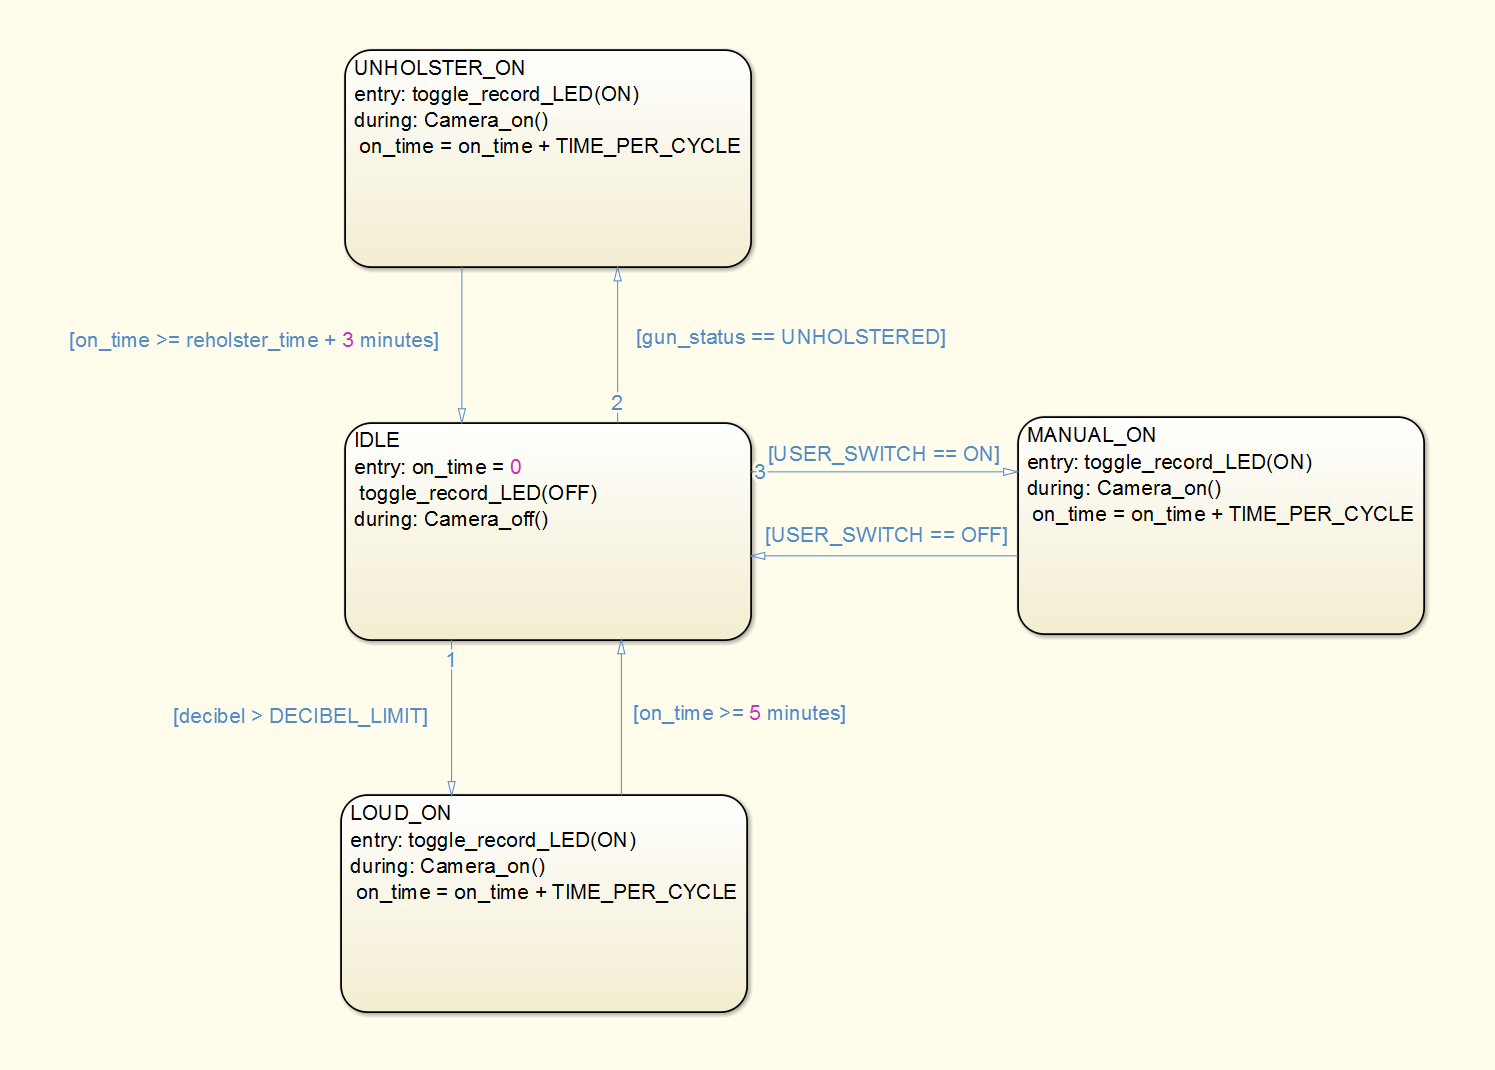
\includegraphics[width=0.9\textwidth]{state_diagram}
    \caption{Camera Record State Diagram}
\end{figure}

For the problem of mounting the camera, we have decided on mounting it on the
officer's shoulder. After reviewing Table \ref{tab:cam_mount} we feel it is
evident that this is the most viable solution. For testing purposes, we do not
need to perform strenuous activity that might cause the shoulder mount to not
capture useful video. We also feel like requiring the officer to wear glasses
would cause problems and we felt like the chest mount would often be obscured
by the way the officer should shoot his weapon.

\begin{figure}[h!]
    \centering
    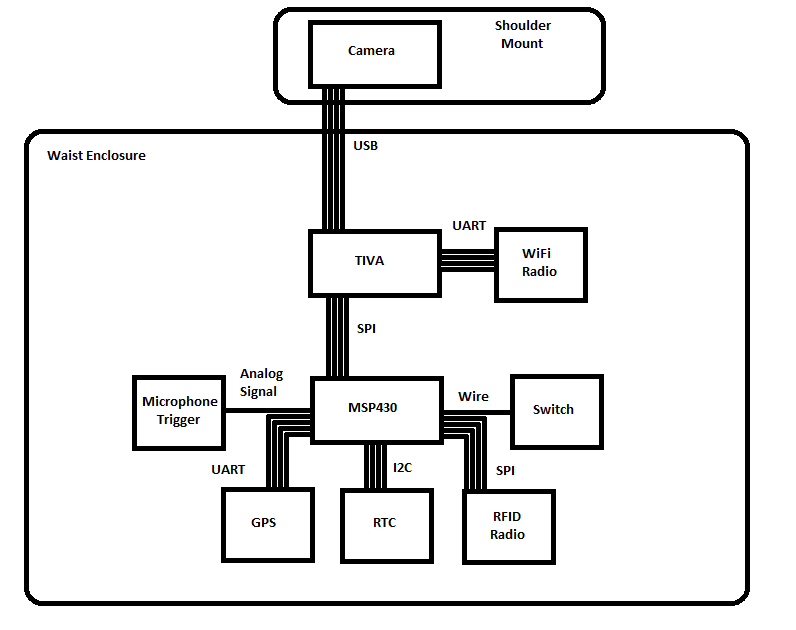
\includegraphics[width=0.9\textwidth]{overview}
    \caption{High Level Overview}
\end{figure}

\section{Power System Design}
Our system is designed to use as little energy as possible by removing power to
all video-related subsystems until video needs to be recorded. The video
subsystem consists of a Texas Instruments TIVA
microcontroller\cite[p.~1880]{tm4c1294ncpdt}, a Texas Instruments CC3000 Wi-Fi
chip\cite[p.~6]{cc3000}, an SD card\cite[p.~19,23]{sd_standard}, a EM-506 GPS
unit\cite[p.~10]{em506}, and a USB camera\cite[p.~245]{usb_standard}. These
parts draw the majority of the power, totalling 4290.4 mW in the worst case.
The rest of the system draws a relatively small 131.4 mW. The individual worst
case power draws are given in Table \ref{tab:worst_case_power}.

% TODO Cite the specification sheets
\begin{table}[h!]
    \centering
    \caption{Worst Case Power Consumption}
    \begin{tabular}{lrrr}
        \textbf{Device} & \textbf{Voltage (V)} & \textbf{Current (mA)} & \textbf{Power (mW)}\\
        TIVA & 3.3 & 133.4 & 440.2\\
        Camera & 5.0 & 500.0 & 2500.0\\
        GPS & 5.0 & 55.0 & 275.0\\
        Microphone & 3.3 & 0.5 & 1.0\\
        RFID Reader & 3.3 & 35.0 & 115.5\\
        SD Card & 3.3 & 100.0 & 330.0\\
        MSP430 & 3.3 & 4.5 & 14.9\\
        CC3000 & 3.6 & 207.0 & 745.2\\
        \hline
        \textbf{Totals} & & & \textbf{Power (mW)}\\
        Idle & & & 131.4\\
        Recording & & & 4421.8\\
    \end{tabular}
    \label{tab:worst_case_power}
\end{table}

In an 8 hour police shift, our device can record up to one half hour of video,
requiring approximately 13.65 Wh of energy. A battery with \textasciitilde{} 20
Wh has been chosen for overhead and to deal with wear in production use. A
lithium-polymer battery was chosen due to the high energy density and ability
to recharge. Lithium-polymer batteries can be dangerous, especially when
exposed to forceful strikes; a tough battery case will mitigate this danger.

\section{Mechanical Design}

The mechanics of this design revolve around one enclosure that contains the PCB
that houses the MSP430, GPS, RTC, RFID reader, an exposed switch, and a
microphone. The RFID reader will have an antenna coming out of the enclosure
that will be mounted on the holster. This enclosure will also contain a TIVA
with an attached WiFi radio, which will also have an externally mounted
antenna. The camera will be mounted on the shoulder of the officer and will be
connected to the enclosure via a USB cable, as the camera solution we have is
USB compatible. The camera will also have an enclosure that allows it to
comfortably be mounted to the officer's shoulder. All connections and the
protocols they use can be found in the diagram above.

Another mechanical design feature is the size limitations we will run into.
However, officers already carry weapons as well as radios on their belt, so
anything we add to the belt will not be too much for the officer as long as it
is not big enough to be physically intrusive. However, sticking to just a
camera mounted on the shoulder is key, because something heavy on a shoulder
could knock his aim off and potentially put the officer in a dangerous
situation. 

\section{Way Forward}

In order to implement our design, we will adhere as closely as possible to the
Gantt chart in Figure \ref{fig:gantt}. The things that are most likely to go
wrong will be developing a streaming driver for video as well as developing the
RFID controller. Our schedule leaves approximately a week to two weeks for
``final manufacturing'', which will be implementing our enclosures and possibly
researching manufacturability and production cost. Manufacturing an enclosure
for our prototype will be fairly simple, because Alec has a lot of experience
working with the 3D printing process. In those few weeks, testing could occur
on any unfinished section of the project. 

\begin{landscape}
    \thispagestyle{empty}

    \begin{figure}[h!]
        \centering
        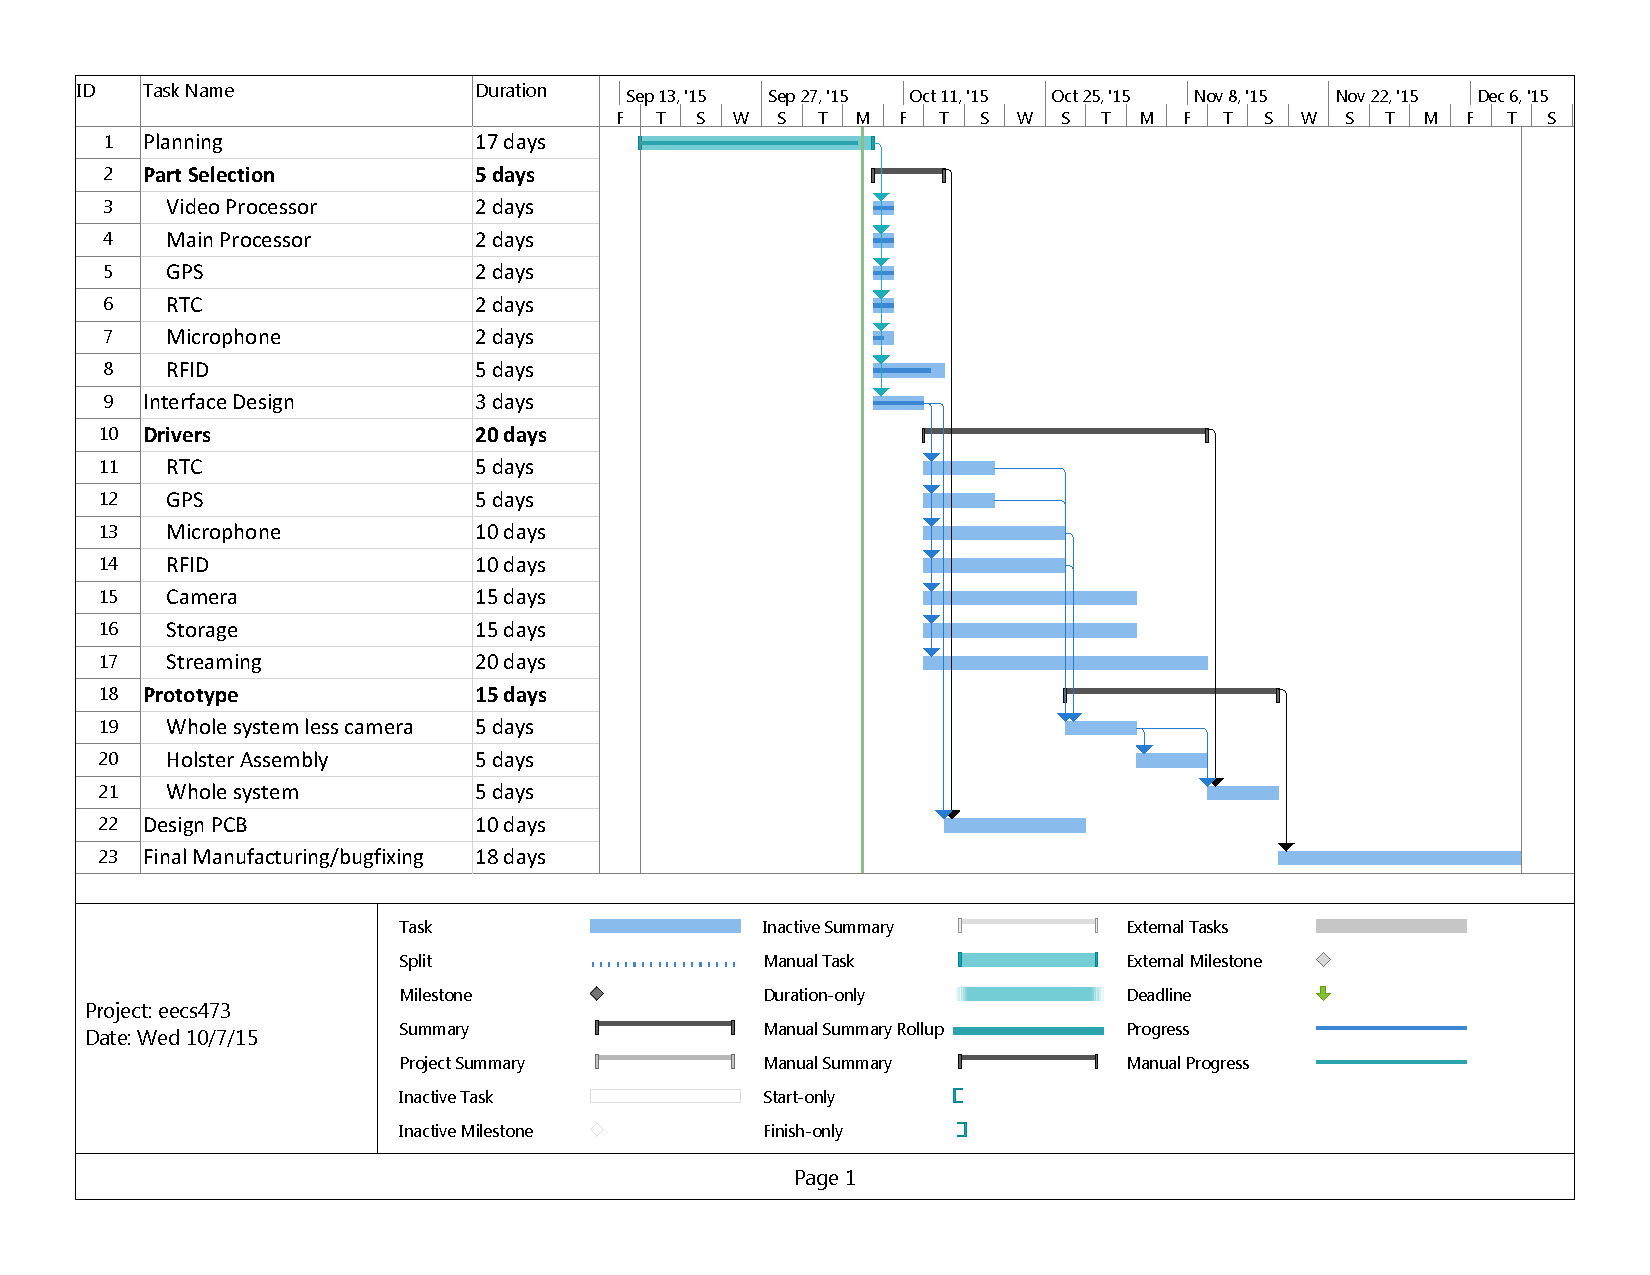
\includegraphics[width=1.2\textwidth]{gantt}
        \caption{Gantt chart}
        \label{fig:gantt}
    \end{figure}
\end{landscape}

\section{Milestones}

\subsection{Milestone 1}

Milestone 1 will be on October 20, where we should have large chunks of many of
the parts of our project done. By this time, we want our MSP430 to generate a
record signal based on volume levels detected by a microphone. The record
signal will also be set by a switch that we interface to, and the RFID reader
will hopefully be close to done.We should have the camera recording and sending
data back to the TIVA, as well as a demo for sending data across a Wifi
connection. The Wifi demo might be as simple as sending one packet with a
string in it, but we will have the connection and that will give us a good
platform for sending over the encoded video data soon after. The MSP430 will
also be reading in GPS and RTC data at a reasonable rate. This data can be
checked via the internet by typing in the coordinates we receive from the
device and checking the time with a clock. 

\subsection{Milestone 2}

Milestone 2 will be on November 4, where we should have the breadboard
prototype completely finished, with video being recorded and streamed over to
the Pi whenever there is a loud noise or the gun is removed from the holster,
as well as if the switch is toggled. All of this will be on a breadboard
prototype, with the PCB having been designed and shipped.  We can all start
testing and designing enclosures, as well as populating and testing our PCB
design.

\section{Budget and Bill of Materials}

\begin{table}[h!]
    \centering
    \caption{Budget}
    \begin{tabular}{lrrlr}
        Product & Cost & Qty & Part & Shipping\\
        Camera & \$37.00 & 1 & Genius F100 & \$0.00\\
        GPS & \$39.95 & 1 & USGlobalSat EM-506 & \$2.50\\
        RTC & \$3.47 & 1 & Epson RX8900CE:UA3 & \$3.00\\
        Microphone & \$7.95 & 1 & CE CEM-C9745JAD462P2.54R & \$2.50\\
        Wifi Radio & \$6.95 & 1 & Nurdspace ESP8266 & \$3.00\\
        RFID Eval Board & donated & 1 & TI EZ430-TMS37157 & \$0.00\\
        Video Eval Board & donated & 1 & TI Tiva & \$0.00\\
        Video Processor & \$15.61 & 1 & TI TM4C1290NCPDT & \$3.04\\
        PCB fabrication & \$33 & 2 & Advanced Circuits & \$10.00\\
        PCB Parts & \$100 & 1 & Digikey & \$20.00\\
        Battery & \$37 & 1 & Venom 3200mAh 20C LiPo & \$0.00\\
        Total & \$312.93 & & & \$44.04\\
    \end{tabular}
\end{table}

\section{Demoables for Design Expo}

Ideally, we will have a base station (a laptop or a Pi) to simulate the squad
cars laptop. The Pi will be a Wifi access point that our wearable will connect
to. From that connection we get a video stream whenever the gun is pulled from
the holster or whenever someone screams or yells near the microphone. We could
also show the hip pack that is tamper-proof. When the gun is not holstered, it
will only show GPS data from the officer’s pack. This could involve possibly
creating a halfway-decent UI, if we have time.

\section{Conclusion}

Our project proposes an optimal scheme to satisfy questions of unethical
conduct by police officers. Even though police officers maintain the right to
apprehend suspects by force, many suspect officers of abuse of their power.
Righteousness of the officers’ actions can not be judged without tangible
evidence of incidents. Having videos recorded only when an incident occurs will
provide tangible evidence to judge whether officers’ actions were just, without
violating officers’ privacy. One of the difficulties is that it is difficult to
precisely distinguish a moment to start recording a video well enough to
encompass whole situation. Achieving live streaming is optimal but will be
challenging to get done in the given scope of the project. However, once our
proposed function is achieved, it will open many possibilities to extend its
uses and functionalities. When successful, this project will provide optimal
functionality for the use of a wearable body camera in a tactical application. 

\newpage

\bibliographystyle{plain}
\bibliography{references}

\newpage

\appendix
\section{Design Criteria}

\begin{table}[h!]
    \centering
    \caption{Design Criteria}
    \begin{tabular}{lll}
        Design Criteria & Importance & Will/Expect/Stretch\\
        RFID/NFC Holster & High & Will\\
        Video Data Saved Locally & High & Will\\
        RTC synced with GPS & High & Will\\
        Holster/Audio Trigger & High & Will\\
        Video Data Streamed & High & Will\\
        Prevent Tampering & Medium & Stretch\\
        Processor on gun for telemetry & Low & Stretch\\
        Mesh Network for multiple Officers & Low & Stretch\\
    \end{tabular}
\end{table}

\newpage

\section{Milestones}

\subsection{Milestone 1}
\begin{itemize}
    \item GPS and RTC tested and verified
    \item Can send a trigger based on sound level or manual switch
    \item RFID in development
    \item Packet can be sent over wifi
    \item Video data verified
\end{itemize}

\subsection{Milestone 2}
\begin{itemize}
    \item Working full-featured prototype, video streamed on any of our triggers
    \item PCB is shipped
    \item Enclosure designed but not printed
\end{itemize}

\newpage

\section{Interface Design}

\begin{lstlisting}
typedef enum day_of_week_t 
{
    SUNDAY,
    MONDAY,
    TUESDAY,
    WEDNESDAY,
    THURSDAY,
    FRIDAY,
    SATURDAY
};


typedef struct rtc_time_t 
{
    uint16_t year;
    uint8_t month;
    day_of_week_t dayOfWeek;
    uint8_t day;
    uint8_t hours;
    uint8_t minutes;
    uint8_t seconds;
};


class RTC_t
{
    public:
    
    void rtcInit();
    rtc_time_t getTime();
    void setTime( rtc_time_t );
    
    private:
    
    rtc_time_t lastTime;
};


typedef enum gps_protocol_t
{
    GPRMC,
    GPGGA,
    GPGSA
};


class GPS_t
{
    public:
    
    void gpsInit();
    void* gpsTask();
    double getLat();
    double getLon();
    rtc_time_t getTime();
    
    private:
    
    gps_protocol_t gpsProtocol;
};


class Wifi_t
{
    public:
    
    void wifiInit();
    int connect();
    int disconnect();
    int send(char* data);
    char* receive();
    
    private:
    int ipAddress;
};


typedef double decibel;


class Microphone_t
{
    public:
    
    void microphoneInit();
    void* microphoneTask();
    decibel getVolume();
    
    private:
};


class Rfid_t
{
    public:
    
    void rfidInit();
    void* rfidTask();
    
    private:
    boolean isTagPresent();
};


class Camera_t
{
    public:
    
    void cameraInit();
    boolean turnCameraOn();
    boolean turnCameraOff();
    boolean isCameraOn();


    private:
};
\end{lstlisting}

\newpage

\section{Group Agreement}

The team will have weekly meetings where all group members are present on
Tuesdays at 7, a time we have all confirmed via WhenIsGood. We will also have
one midday meeting during the weekend, either Saturdays or Sundays that are
fairly informal where we meet for lunch and discuss high level project goals
and problems. Most meetings will take place in the MESH or 473 lab.. The team
has a WhenIsGood in order to organize meeting times for tasks involving two or
more people, but team members are expected to get work done on their own as
well. The group has its own email at 473.body.cam@umich.edu, as well as a
GroupMe we use to send text message updates to each other. Most of the work
will be done in the 473 lab, but any PCB work will probably be done in the MESH
lab. Any 3D printing will be done in the AERO lab. We also have designated who
will be working on which parts of the project, based on each group member’s
individual strengths. We expect the group members to spend approximately 25-30
hours per week at the beginning of the project, and approximately 40 hours per
week during the second half until the end of the project. The task list is as
follows:

Known Conflicts:

\ \\

\begin{tabular}{lll}
    Who & What & When\\
    All & Fall Study Break & October 17-20\\
    All & 473 Midterm & October 27\\
    All & Thanksgiving Break & November 25-30\\
    Alex & Out of town & October 25\\
    Alex & Out of town & November 5\\
    Alec & Wisdom Teeth Removal & October 20-22\\
    Yun & Out of town & October 9\\
\end{tabular}

\begin{itemize}
    \item Meeting Minutes - Alex
    \item Group Coordination - Jake
    \item Real Time Clock - Jake
    \item GPS - Alex
    \item RFID Reader - Yun
    \item Microphone - Alex
    \item Camera \begin{itemize}
            \item LED - Alec/Jiqing
            \item Storage - Alec/Jiqing
            \item Low Level Interface - Alec/Jiqing
            \item Streaming - Alex
        \end{itemize}
    \item Mech. CAD and 3D printing - Alex/Alec
    \item PCB Design - Jake/Jiqing
\end{itemize}

\end{document}
